\section{Loss functions for multiple annotators}

As mentioned in Section \ref{sec:architecture_and_training}, a loss
function is a key element for defining the objective function of a
deep learning model. The categorical cross-entropy loss is a common
loss function for classification tasks. However, in the case of
multiple annotators, the categorical cross-entropy loss is not able
to handle the varying reliability of the annotators. In this section,
we will propose a loss function that is able to handle multiple
annotators' segmentation masks while accounting for their varying reliability
across different regions of the image.

\subsection{Generalized Cross Entropy}

The \gls{GCE} loss function was first introduced by
\cite{ZhangEtAl2018} as a robust alternative to the standard
cross-entropy loss, particularly effective in handling noisy labels.
Let us first consider the \gls{CE} and \gls{MAE} loss functions:

\begin{equation}
  MAE(\mathbf{y}, f(\mathbf{x})) = \|\mathbf{y} - f(\mathbf{x})\|_1
\end{equation}

\begin{equation}
  CE(\mathbf{y}, f(\mathbf{x})) = \sum_{k=1}^K y_k \log(f_k(\mathbf{x}))
\end{equation}

where $y_k \in \mathbf{y}$, $f_k(\mathbf{x}) \in f(\mathbf{x})$, and
$\|\cdot\|_1$ stands for the $l_1$-norm. Of note,
$\mathbf{1}^\top\mathbf{y} = \mathbf{1}^\top f(\mathbf{x}) = 1$,
$\mathbf{1} \in \{1\}^K$ being an all-ones vector. In addition, the
MAE loss can be rewritten for softmax outputs, yielding:

\begin{equation}
  MAE(\mathbf{y}, f(\mathbf{x})) = 2(1 - \mathbf{1}^\top(\mathbf{y}
  \odot f(\mathbf{x})))
\end{equation}

where $\odot$ stands for the element-wise product.

The \gls{CE} loss function exhibits several distinct characteristics
that make it particularly sensitive to noisy labels. It is unbounded
from above and heavily penalizes confident but wrong predictions,
which can lead to instability in the presence of label noise. In
contrast, the \gls{MAE} loss offers a more robust alternative with
its bounded nature and symmetric properties in softmax-based
representations. While the MAE loss is more resilient to noisy
labels, it tends to train more slowly due to its equal weighting of
all mistakes regardless of confidence.

The GCE loss function, as defined by the authors in
\cite{ZhangEtAl2018}, provides a flexible framework that bridges
these two approaches:

\begin{equation}
  GCE(\mathbf{y}, f(\mathbf{x})) = 2\frac{1 -
  (\mathbf{1}^\top(\mathbf{y} \odot f(\mathbf{x})))^q}{q},
\end{equation}

with $q \in (0,1]$. Remarkably, the limiting case for $q \to 0$ in
GCE is equivalent to the CE expression, and when $q = 1$, it equals
the MAE loss. In addition, the GCE holds the following gradient with
regard to $\theta$:

\begin{equation}
  \frac{\partial GCE(\mathbf{y}, f(\mathbf{x};\theta)|k)}{\partial
  \theta} = -f_k(\mathbf{x};\theta)^{q-1}\nabla_\theta f_k(\mathbf{x};\theta).
\end{equation}

The GCE loss combines the best of both worlds, offering robustness to
label noise while maintaining the convexity property necessary for
optimization. The truncation parameter $q$ provides a mechanism to
control the sensitivity to outliers, allowing for fine-tuning of the
loss function's behavior based on the specific characteristics of the dataset.

\subsection{Extension to Multiple Annotators}

In the context of multiple annotators, we need to consider the
varying reliability of each annotator across different regions of the
image. Let's consider a $k$-class multiple annotators segmentation
problem with the following data representation:

\begin{equation}
  \mathbf X \in \mathbb{R}^{W \times H}, \{ \mathbf Y_r \in
  \{0,1\}^{W \times H \times K} \}_{r=1}^R; \;\; \mathbf {\hat Y} \in
  [0,1]^{W\times H \times K} = f(\mathbf X)
\end{equation}

where the segmentation mask function maps the input to output as:

\begin{equation}
  f: \mathbb  R ^{W\times H} \to [0,1]^{W\times H\times K}
\end{equation}

The segmentation masks $\mathbf Y_r$ satisfy the following condition
for being a softmax-like representation:

\begin{equation}
  \mathbf Y_r[w,h,:] \mathbf{1} ^ \top _ k = 1; \;\; w \in W, h \in H
\end{equation}

\subsection{Reliability Maps and Truncated GCE}

The key innovation in our approach is the introduction of reliability
maps $\Lambda_r$ for each annotator:

\begin{equation}
  \bigg\{ \Lambda_r (\mathbf X; \theta ) \in [0,1] ^{W\times H} \bigg\}_{r=1}^R
\end{equation}

These reliability maps serve as a sophisticated mechanism to estimate
the confidence of each annotator at every spatial location $(w,h)$ in
the image. By learning these maps jointly with the segmentation
model, the network gains the ability to adapt to the varying levels
of expertise across different regions of the image. This approach
allows for dynamic weighting of each annotator's contribution based
on their estimated reliability in specific areas, effectively
handling cases where annotators might demonstrate different levels of
expertise in different parts of the image.

The proposed Truncated Generalized Cross Entropy for Semantic
Segmentation (TGCE$_{SS}$) combines the robustness of GCE with the
flexibility of reliability maps:

\begin{equation}
  \begin{split}
    TGCE_{SS}(\mathbf{Y}_r,f(\mathbf X;\theta) | \mathbf{\Lambda}_r
    (\mathbf X;\theta)) = \mathbb E_{r} \Bigg\{ \mathbb E_{w,h}
      \Bigg\{ \Lambda_r (\mathbf X; \theta) \circ \mathbb E_k \bigg\{
          \mathbf Y_r \circ \bigg( \frac{\mathbf 1 _{W\times H \times
        K} - f(\mathbf X;\theta) ^{\circ q }}{q} \bigg); k \in K  \bigg\}  + \\
        \left(\mathbf 1 _{W \times H } - \Lambda _r (\mathbf
        X;\theta)\right) \circ \bigg(   \frac{\mathbf 1_{W\times H} -
        (\frac {1}{k} \mathbf 1_{W\times H})^{\circ q}}{q} \bigg); w \in
    W, h \in H \Bigg\};r\in R\Bigg\}
  \end{split}
\end{equation}

where $q \in (0,1)$ controls the \gls{MAE} or \gls{CE} level in the
same way as in the \gls{GCE} loss function. The loss function consists of
two main components:

\begin{itemize}
  \item The first term weighted by $\Lambda_r$ represents the GCE
    loss for regions where the annotator is considered reliable
  \item The second term weighted by $(1-\Lambda_r)$ provides a
    uniform prior for regions where the annotator is considered unreliable
\end{itemize}

For a batch containing $N$ samples, the total loss is computed as:

\begin{equation}
  \mathscr{L}\left(\mathbf{Y}_r[n],f(\mathbf X[n];\theta) |
  \mathbf{\Lambda}_r (\mathbf X[n];\theta)\right)  = \frac{1}{N}
  \sum_{n}^N TGCE_{SS}(\mathbf{Y}_r[n],f(\mathbf X[n];\theta) |
  \mathbf{\Lambda}_r (\mathbf X[n];\theta))
\end{equation}

\begin{figure}[t]
  \centering
  \begin{tikzpicture}[
      node distance=1.5cm,
      block/.style={rectangle, draw, minimum width=1cm, minimum
      height=1cm, text centered},
      arrow/.style={->, >=stealth},
      label/.style={text width=2cm, align=center}
    ]

    % Input image
    \node[block] (input) {
    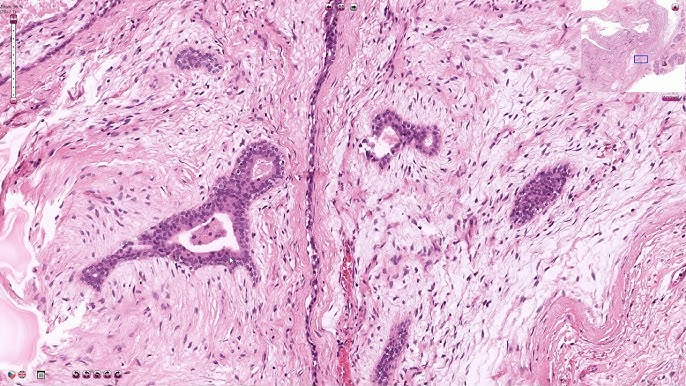
\includegraphics[width=2cm]{Cap4/Figures/histopathology_patch.jpg}};
    \node[text width=2cm, align=center, above of=input, yshift=0.5cm]
    {Input Image $\mathbf{X}$};

    % Annotator masks
    \node[block, right of=input, xshift=2cm] (mask1) {$\mathbf{Y}_1$};
    \node[block, above of=mask1] (mask2) {$\mathbf{Y}_2$};
    \node[block, below of=mask1] (mask3) {$\mathbf{Y}_R$};

    % Reliability maps
    \node[block, right of=mask1, xshift=1cm] (rel1) {$\Lambda_1$};
    \node[block, right of=mask2, xshift=1cm] (rel2) {$\Lambda_2$};
    \node[block, right of=mask3, xshift=1cm] (rel3) {$\Lambda_R$};

    % Model prediction
    \node[block, right of=rel1, xshift=2cm] (pred) {$f(\mathbf{X};\theta)$};

    % Loss computation
    \node[block, below of=pred, yshift=-2cm] (loss) {TGCE$_{SS}$ Loss};

    % Arrows
    \draw[arrow] (input) -- (mask1);
    \draw[arrow] (input) -- (mask2);
    \draw[arrow] (input) -- (mask3);

    \draw[arrow] (mask1) -- (rel1);
    \draw[arrow] (mask2) -- (rel2);
    \draw[arrow] (mask3) -- (rel3);

    \draw[arrow] (rel1) -- (loss);
    \draw[arrow] (rel2) -- (loss);
    \draw[arrow] (rel3) -- (loss);
    \draw[arrow] (pred) -- (loss);

    % Annotations
    \node[text width=2cm, align=center, above of=mask2, yshift=0.5cm]
    {Annotator Masks};
    \node[text width=2cm, align=center, above of=rel2, yshift=0.5cm]
    {Reliability Maps};
    \node[text width=2cm, align=center, above of=pred, yshift=0.5cm]
    {Model Prediction};

    % Loss components
    \node[block, below of=loss, yshift=-3cm] (reliable) {Reliable Regions Loss};
    \node[block, left of=reliable, xshift=-3cm] (unreliable)
    {Unreliable Regions Loss};

    \draw[arrow] (loss) -- (reliable);
    \draw[arrow] (loss) -- (unreliable);

    % Legend
    \node[text width=4cm, align=left, right of=loss, xshift=2cm] {
      \textbf{Loss Components:}\\
      $\bullet$ Reliable: $\Lambda_r \circ GCE$\\
      $\bullet$ Unreliable: $(1-\Lambda_r) \circ \text{Uniform Prior}$
    };

  \end{tikzpicture}
  \caption{Working mechanism of the proposed Truncated Generalized
    Cross Entropy for Semantic Segmentation (TGCE$_{SS}$) loss
    function. The loss combines reliability maps $\Lambda_r$ with the
    model's predictions $f(\mathbf{X};\theta)$ to compute a weighted
  loss that accounts for annotator reliability across different image regions.}
  \label{fig:loss_mechanism}
\end{figure}